\newpage

\section{Foundations of Data Flow Analysis}



We saw a lot of examples of data flow analysis, eg. reaching definitions etc. Although
there were differences between differeent types of data flow analysis, they did share number of
things in common. Our goal is to develop a general purpose data flow analysis framework.


There are some questions that we want to answer about a framework that performs data
flow analysis.

\begin{itemize}
	\item Correctness: Do we get a correct answer?
	\item Precison: How good is the answer? \footnote{We want a safe solution but as precise as possible. }
	\item Covergence: Will the analysis terminate?
	\item Speed: How fast is the convergence?
\end{itemize}



\subsection{A Unified Framework}

Data flow problems are defined by
\begin{itemize}

	\item Domain of values \( V \)(eg, variable names for liverness, the instruction numbers for reaching definitions)
	\item Meet operator \( V \wedge V \rightarrow V \) to deal with the join nodes.
	\item Initial value. Once we have defined the meet operator, it will tell us how to initialize
	      all of the non-entry or exits nodes and the boundary conditions for entry and exit nodes.
	\item A set of transfer functions \( V  \rightarrow V \) to define how information flows across basic blocks.
\end{itemize}



Why we bother to define such a framework?
\begin{itemize}
	\item First, if meet operator, transfer function and the domains of values are specified in proper way, we will know about
	      correctness, precision and so on.

	\item From practical engineering perspective, it allows us to reuse code.
\end{itemize}


\subsection{Partial Order}

A relation \(R\) on a set \(S\) is called a \textbf{partial order} if it is

\begin{itemize}
	\item \textbf{Transitivity} if \(x \preceq y\) and  \(y \preceq z\) then  \(x \preceq z\)
	\item \textbf{Antisymmetriy} if \(x \preceq y\) and  \(y \preceq x\) then  \(x = x\)
	\item \textbf{Reflexivity}  \(x \preceq x\)
\end{itemize}

\subsection{Lattice}

A lattice is a partially ordered set in which every pair of elements has both a least upper bound (lub)
and a greatest lower bound(glb).

\begin{figure}[h]
	\centering
	\begin{subfigure}[b]{0.3\textwidth}
		\centering
		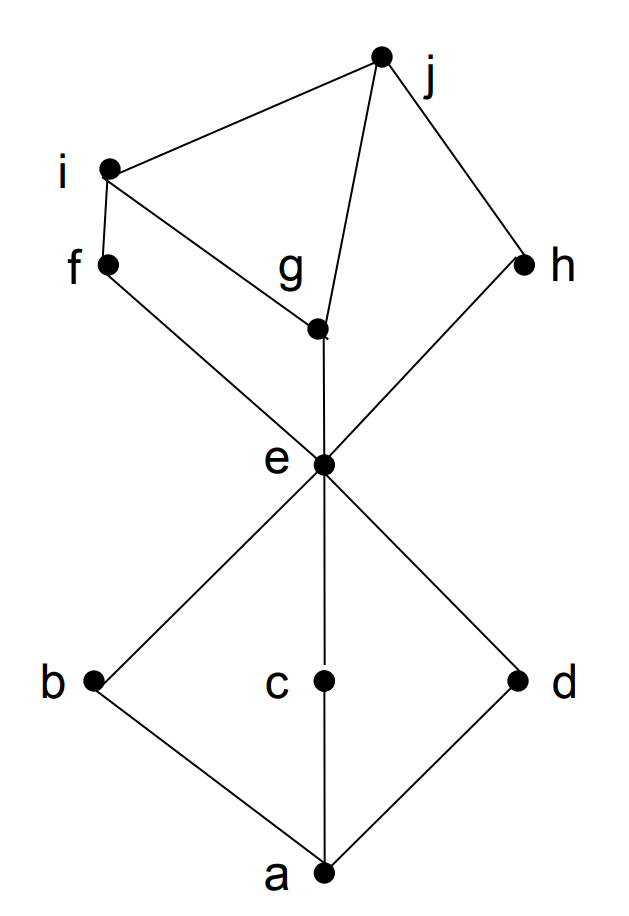
\includegraphics[width=\textwidth]{p17.png}
		\caption{This is a lattice example.}
		\label{fig:p17}
	\end{subfigure}
	\hfill
	\begin{subfigure}[b]{0.3\textwidth}
		\centering
		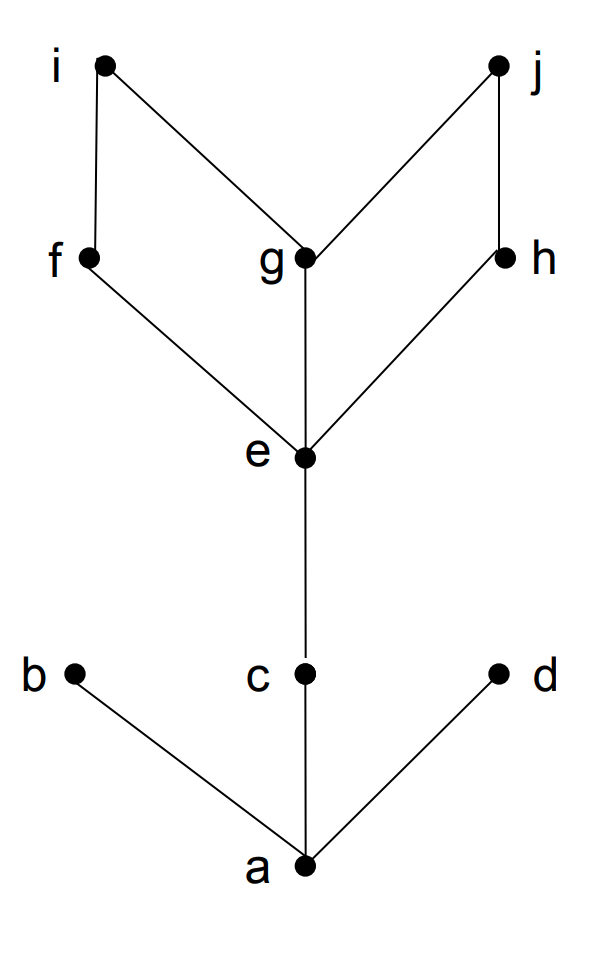
\includegraphics[width=\textwidth]{p16.png}
		\caption{This is not a lattice example becuasethe pair {b,c} deos not have a lub.}
		\label{fig:three sin x}
	\end{subfigure}
	\caption{Two examples}
	\label{fig:p16}
\end{figure}





\subsection{Complete Lattice}

A lattice A is called a complete lattice if every subset S of A admits a
glb and a lub in A.



\subsection{Semi-Lattice}

A semilattice (or upper semilattice) is a partially ordered set that has a least upper bound for any
nonempty finite subset.





\subsection{ Meet Operator }

Meet operator must hold the following properties:

\begin{itemize}
	\item \textbf{commutative}: \(x \wedge y = y  \wedge x\). No ordering in the incoming edges.

	\item \textbf{idempotent}: \(x \wedge x =  x\)

	\item \textbf{associative }: \(x \wedge( y\wedge z) =  (x \wedge y) \wedge z\)

	\item there is a Top element T such that \(x \wedge T = x\). Partly due to the way
	      we initialize everything we need.
\end{itemize}

\begin{figure}[h]
	\centering
	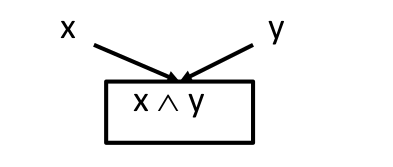
\includegraphics[width=0.3\textwidth]{p15.png}
	\caption{Meet Operator}
	\label{fig:p15}
\end{figure}



Meet Operator defines a partial ordering on values. This is important in ensuring the analysis converges. So
what does it mean ? \(x \preceq y\) if and only if \(x \wedge y = x\). The \(\preceq \) not means less or equal to or subset, but it really means lattice inclusion.
So if \(x \preceq y\), this means x is more conservative or constrained. In another word, x is lattice included in y.
Partial  ordering will also lead to some other properties
\begin{itemize}
	\item \textbf{Transitivity} if \(x \preceq y\) and  \(y \preceq z\) then  \(x \preceq z\)
	\item \textbf{Antisymmetriy} if \(x \preceq y\) and  \(y \preceq x\) then  \(x = z\)
	\item \textbf{Reflexivity}  \(x \preceq x\)
\end{itemize}


\begin{figure}[h]
	\centering
	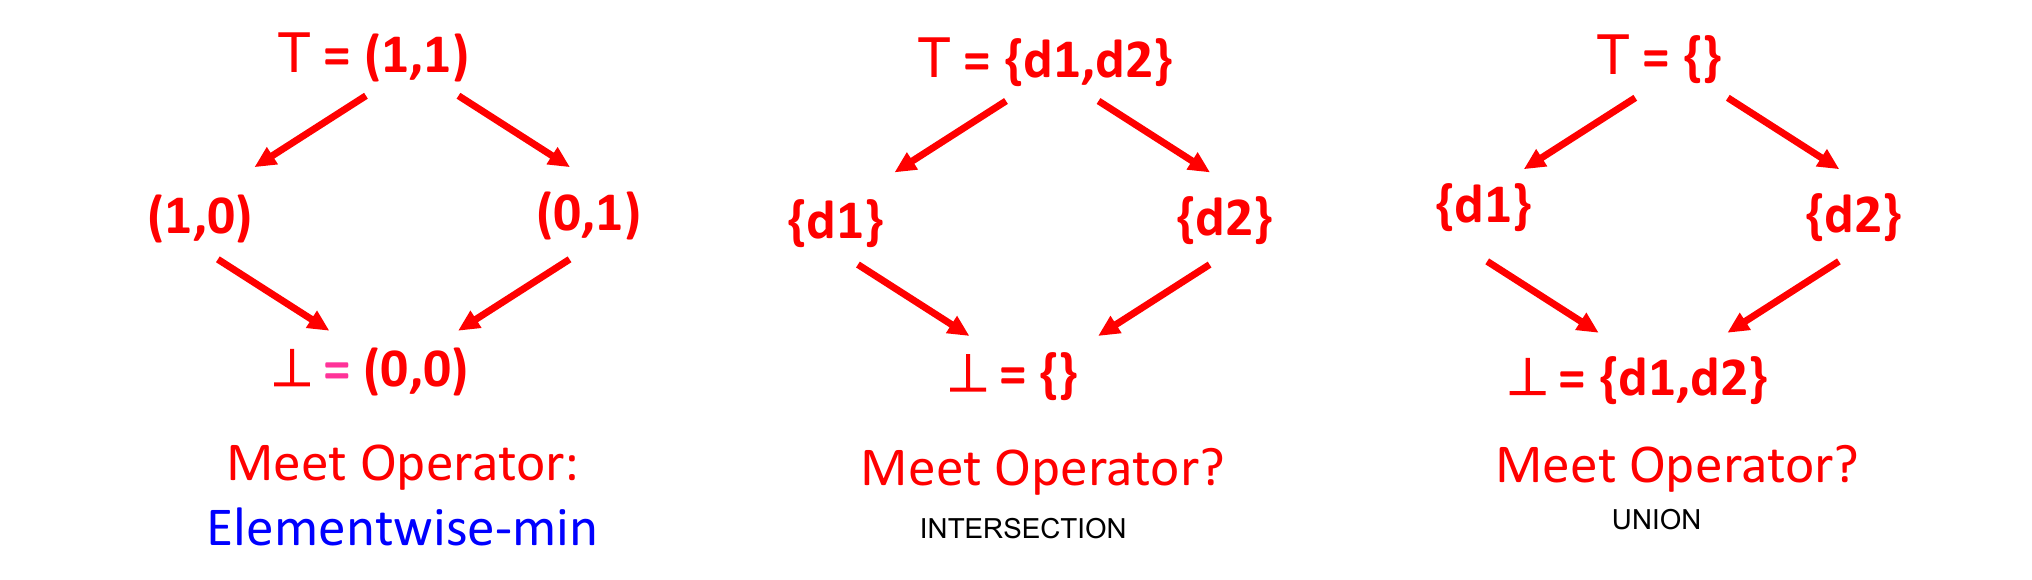
\includegraphics[width=\textwidth]{p18.png}
	\caption{Different meet operator defines different lattice}
	\label{fig:p15}
\end{figure}


% \subsection{Partial Order}


For our data flow analysis, values and meet operator define a semi-lattice, which means \(\top\) exits, but not necessarily \(	\bot\).





\subsection{Descending Chain}

The height of a lattice is the largest number of \(\succ \) relations that will fit in a descending chain. eg. \(x_0 \succ x_1 \succ x_2 \succ \dots\)

So, for reaching definitions, the height is the number of definitions.

Finite descending chain will ensure the convergence. If we don't finite descending chain, there is a possibility that
the analysis will never terminate. But a infinite lattice still can have a finite descending chain. I want to note that
infinite lattice doesn't always mean a non-convergence.

So consider the constant propogation, the infinite lattice has finite descending chain, so this can converge.

\begin{figure}[h]
	\centering
	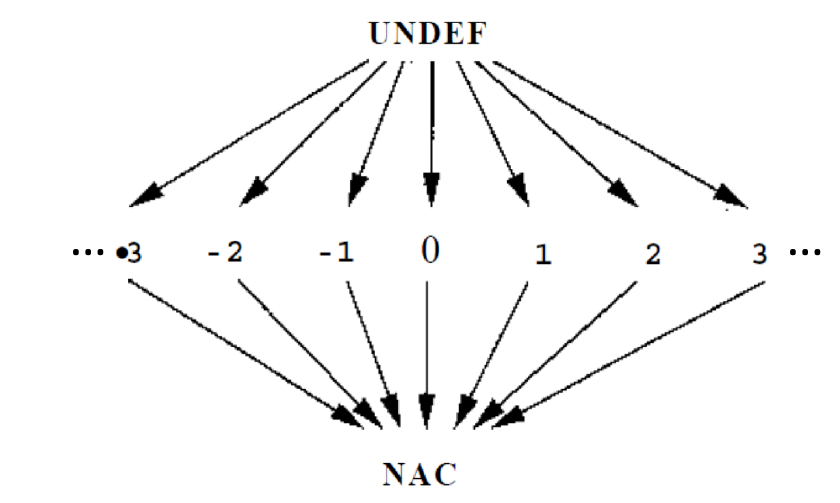
\includegraphics[width=0.3\textwidth]{p19.png}
	\caption{The lattice of constant propogation}
	\label{fig:p19}
\end{figure}


\subsection{Transfer Functions}

Tranfer function dicates how information propagates across a basic block.
So what we need for our transfer function? \textbf{First}, it must have an identity function which means
there exists an \(f\) such that \(f(x) = x \) for all \(x\). For example, in Reaching Definitions and Liveness, when
\(Gen, KILL = \Phi \), this transfer function satisfies \(f(x) = x \). \textbf{Second}, when we compose transfer functions,
it must be consitent with the transfer function. So if \(f_1,f_2 \in F\), the  \(f_1	\cdot f_2 \in F\).


For example,
\begin{align*}
	f_1(x)      & = G_1 \cup (x - K_1)                             \\
	f_2(x)      & = G_2 \cup (x - K_2)                             \\
	f_2(f_1(x)) & = G_2 \cup [(G_1 \cup (x - K_1)) - K_2]          \\
	            & = [G_2 \cup (G_1 - K_2)] \cup [x-(K_1 \cup K_2)] \\
	G           & = G_2 \cup (G_1 - K_2)                           \\
	K           & = K_1 \cup K_2
\end{align*}


\subsection{Monotonicity}


A framework \((F,V,\wedge)\) is monotone if and only if \(x \preceq y \) implies \(f(x) \preceq f(y)\). This means that
a "smaller(more conservative) or equal" input to the same function will always give a "smaller(more conservative)  or equal" output.



Alternatively, \((F,V,\wedge)\) is monotone if and only if \(  f(x \wedge y) \preceq f(x) \wedge f(y)\). So  merge input, then apply \(f\) is small(more conservative)  or equal to apply the transfer
function individually and then merge the result. Values are defined by semi-lattice, the meet operator only ever moves down the lattice from top towards the bottom.
So we need to constrain the transfer function.

I will show you a unmonotone example.

Let top be 1 and bottom be 0 and the meet operator is \(\cap\). \(f(0) = 1, f(1) = 0\)


Let's check whether reaching definitions is monotone.


Note that monotone framework does not mean \(f(x) \preceq  x\).



\subsection{Distributivity}

A framework \((F,V,\wedge)\) is distributive if and only if it

\[
	f(x \wedge y) = f(x) \wedge f(y)
\]



Reaching definitions is distributive but constant propogation is not.




\subsection{Defining a Dataflow Problem}


Before thinking about how to define a dataflow problem, note that there are two kinds of problems:
\begin{itemize}
\item Forward problems (like constant propagation) where the information at a node n summarizes what can happen on paths from "enter" to n.
\item Backward problems (like live-variable analysis), where the information at a node n summarizes what can happen on paths from n to "exit".


\end{itemize}	
In what follows, we will assume that we're thinking about a forward problem unless otherwise specified.

Another way that many common dataflow problems can be categorized is as 
may problems or must problems. The solution to a "may" problem provides 
information about what may be true at each program point 
(e.g., for live-variables analysis, a variable is considered live after 
node n if its value may be used before being overwritten, 
while for constant propagation, the pair (x, v) holds before node n if x
 must have the value v at that point).

Now let's think about how to define a dataflow problem so that it's 
clear what the (best) solution should be. When we do dataflow analysis 
"by hand", we look at the CFG and think about:

\begin{itemize}
	\item 	What information holds at the start of the program.
	\item 	When a node n has more than one incoming edge in the CFG, how to combine the incoming information (i.e., given the information that holds after each predecessor of n, how to combine that information to determine what holds before n).
	\item 	How the execution of each node changes the information.
	
\end{itemize}	
This intuition leads to the following definition. An instance of a dataflow problem includes:


\begin{itemize}
	\item a CFG,
	\item a domain D of "dataflow facts",
	\item a dataflow fact "init" (the information true at the start of the program for forward problems, or at the end of the program for backward problems),
	\item an operator $\wedge$ (used to combine incoming information from multiple predecessors),
	\item for each CFG node n, a dataflow function $f_n : D \rightarrow D$ (that defines the effect of executing n).
			
\end{itemize}	

For constant propagation, an individual dataflow fact is a set of pairs of the form (var, val), so the domain of dataflow facts is the set of all such sets of pairs (the power set). For live-variable analysis, it is the power set of the set of variables in the program.

For both constant propagation and live-variable analysis, the "init" fact is the empty set (no variable starts with a constant value, and no variables are live at the end of the program).

For constant propagation, the combining operation $\wedge$ is set intersection. This is because if a node n has two predecessors, p1 and p2, then variable x has value v before node n iff it has value v after both p1 and p2. For live-variable analysis, $\wedge$ is set union: if a node n has two successors, s1 and s2, then the value of x after n may be used before being overwritten iff that holds either before s1 or before s2. In general, for "may" dataflow problems, $\wedge$ will be some union-like operator, while it will be an intersection-like operator for "must" problems.

For constant propagation, the dataflow function associated with a CFG node that does not assign to any variable (e.g., a predicate) is the identity function. For a node n that assigns to a variable x, there are two possibilities:
\begin{itemize}
\item The right-hand side has a variable that is not constant. In this case, the function result is the same as its input except that if variable x was constant the before n, it is not constant after n.
\item All right-hand-side variables have constant values. In this case, the right-hand side of the assignment is evaluated producing consant-value c, and the dataflow-function result is the same as its input except that it includes the pair (x, c) for variable x (and excludes the pair for x, if any, that was in the input).

\end{itemize}	
For live-variable analysis, the dataflow function for each node n has 
the form: $f_n(S) = (S - KILL_n)  \cup  GEN_n$, where $KILL_n$
 is the set of variables defined at node n, and $GEN_n$ is the set 
 of variables used at node n. In other words, for a node
  that does not assign to any variable, the variables that
   are live before n are those that are live after n plus those 
   that are used at n; for a node that assigns to variable x, the 
   variables that are live before n are those that are live after 
   n except x, plus those that are used at n (including x if it 
   is used at n as well as being defined there).


   
It turns out that a number of interesting dataflow problems 
have dataflow functions of this same form, where $GEN_n$ and $KILL_n$
 are sets whose definition depends only on n, and the combining 
 operator $\wedge$ is either union or intersection. These problems 
 are called GEN/KILL problems, or bit-vector problems.

\subsection{Meet-Over-Paths(MOP)\cite{DATAFLOW66:online}}

A solution to an instance of a dataflow problem is a dataflow fact for each node of the given CFG. But what does it mean for a solution to be correct, and if there is more than one correct solution, how can we judge whether one is better than another?

Ideally, we would like the information at a node to reflect what might happen on all possible paths to that node. This ideal solution is called the meet over all paths (MOP) solution, and is discussed below. Unfortunately, it is not always possible to compute the MOP solution; we must sometimes settle for a solution that provides less precise information.


The MOP solution (for a forward problem) for each CFG node n is defined as follows:


\begin{itemize}
	\item For every path "enter $\rightarrow$  $\cdots$  $\rightarrow$ n", compute the dataflow fact induced by that path
	      (by applying the dataflow functions associated with the nodes on the path to the initial dataflow fact).
	\item Combine the computed facts (using the combining operator, $\wedge $ ).
	\item The result is the MOP solution for node n.

\end{itemize}


It is worth noting that even the MOP solution can be overly conservative
(i.e., may include too much information for a "may" problem, and too little information for a "must" problem),
because not all paths in the CFG are executable. For example, a program may include a predicate that always evaluates to false
(e.g., a programmer may include a test as a debugging device -- if the program is correct, then the test will always fail,
but if the program contains an error then the test might succeed, reporting that error). Another way that non-executable paths
can arise is when two predicates on the path are not independent (e.g., whenever the first evaluates to true then so does the second).
These situations are illustrated in Figure \ref{fig:p209}.



\begin{figure}[H]
	\centering
	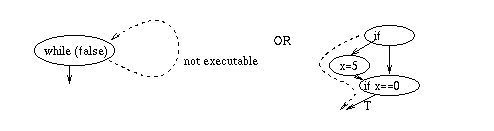
\includegraphics[width=0.8\textwidth]{p209.png}
	\caption{Examples to illustrate MOP is overly conservative.}
	\label{fig:p209}
\end{figure}




So $\mathrm{MOP} = {\color{red}\mathrm{Perfect-Solution   }} \,\,\,U\,\,\, {\color{red}\mathrm{   Solution-to-Unexecuted-Paths}}$

Unfortunately, since most programs include loops, they also have infinitely many paths, and thus it is not possible to
compute the MOP solution to a dataflow problem by computing information for every path and combining that information. Fortunately,
there are other ways to solve dataflow problems (given certain reasonable assumptions about the dataflow functions associated with
the CFG nodes). As we shall see, if those functions are distributive, then the solution that we compute is identical to the MOP
solution. If the functions are monotonic, then the solution may not be identical to the MOP solution, but is a conservative
approximation.

\subsection{Solving a Dataflow Problem by Solving a Set of Equations}

The alternative to computing the MOP solution directly, is to solve a system of equations
that essentially specify that local information must be consistent with the dataflow functions.
In particular, we associate two dataflow facts with each node n:
\begin{itemize}
	\item \textit{n.before}: the information that holds before n executes, and
	\item \textit{n.after}: the information that holds after n executes.
\end{itemize}

These \textit{n.before}s and \textit{n.after}s are the variables of our equations,
which are defined as follows (two equations for each node n):


\begin{itemize}
	\item \textit{n.before} = $\wedge$(\textit{p1.after, p2.after}, ...)
	      where p1, p2, etc are n's predecessors in the CFG (and $\wedge$ is the
	      combining operator for this dataflow problem).
	\item \textit{n.after} = $f_n$(\textit{n.before})
\end{itemize}

In addition, we have one equation for the enter node:

\begin{itemize}

	\item \textit{enter.after = init} (recall that "init" is part of the specification of a dataflow problem)
\end{itemize}

These equations make intuitive sense: the dataflow information that holds
before node n executes is the combination of the information that holds after
each of n's predecessors executes, and the information that holds after n
executes is the result of applying n's dataflow function to the information
that holds before n executes.

One question is whether, in general, our system of equations will have a
unique solution. The answer is that, in the presence of loops, there may
be multiple solutions. For example, consider the simple program whose CFG
is given in Figure \ref{fig:p215}:


\begin{figure}[H]
	\centering
	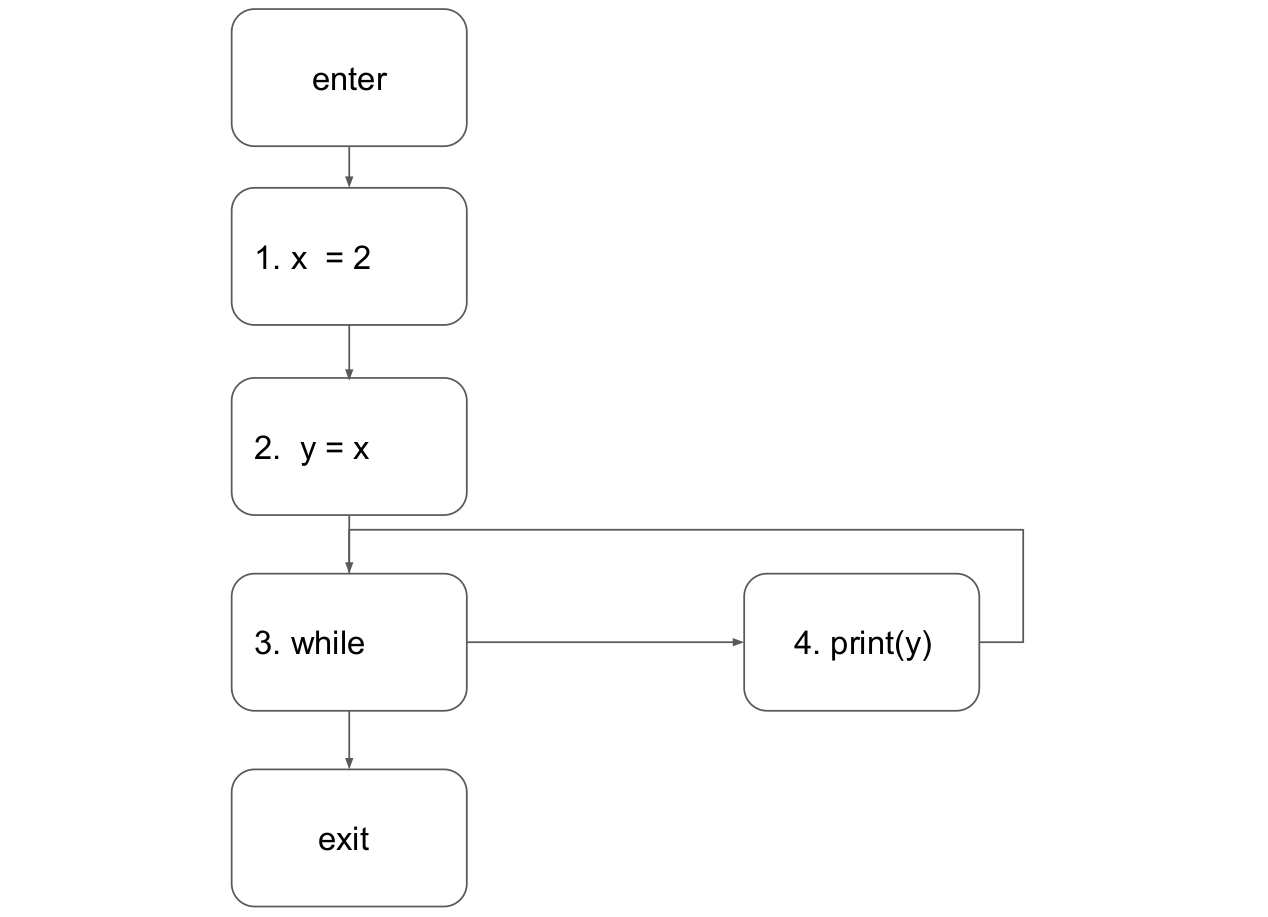
\includegraphics[width=0.4\textwidth]{p215.png}
	\caption{An example to illustrate the system of equations.}
	\label{fig:p215}
\end{figure}

The equations for constant propagation are as follows:\\
{
\texttt{enter.after} $= \Phi $ \\
\texttt{1.before} $=$  \texttt{enter.after} \\
\texttt{1.after} $=$ \texttt{1.before} $-(x, *)$ {\color{red} union} $(x, 2)$  \\
\texttt{2.before} $=$ \texttt{1.after} \\
\texttt{2.after} $=$ if $(x, c)$ is in  \texttt{2.before} then  \texttt{2.before} $-(y, *)$ {\color{red} union} $(y, c)$, else  \texttt{2.before} $-(y, *)$  \\
\texttt{3.before} $= \wedge $ ( \texttt{2.after, 4.after} ) \\
\texttt{3.after} $=$  \texttt{3.before} \\
\texttt{4.before} $=$  \texttt{3.after} \\
\texttt{4.after} $=$  \texttt{4.before} \\
}
Because of the cycle in the example CFG, the equations for  \texttt{3.before,
	3.after, 4.before, and 4.after} are mutually recursive, which leads to the
four solutions shown below (differing on those four values).

$$
	\begin{array}{|c|c|c|c|c|}
		\hline \text { Variable }        & \text { Solution 1 } & \text { Solution 2 } & \text { Solution 3 } & \text { Solution 4 } \\
		\hline  \text { 1.before } & \{\}                 & \{\}                 & \{\}                 & \{\}                 \\
		\hline  \text { 1.after }  & \{(x, 2)\}           & \{(x, 2)\}           & \{(x, 2)\}           & \{(x, 2)\}           \\
		\hline  \text { 2.before } & \{(x, 2)\}           & \{(x, 2)\}           & \{(x, 2)\}           & \{(x, 2)\}           \\
		\hline  \text { 2.after }  & \{(x, 2)(y, 2)\}     & \{(x, 2)(y, 2)\}     & \{(x, 2)(y, 2)\}     & \{(x, 2)(y, 2)\}     \\
		\hline  \text { 3.before } & \{\}                 & \{(x, 2)\}           & \{(y, 2)\}           & \{(x, 2)(y, 2)\}     \\
		\hline  \text { 3.after }  & \{\}                 & \{(x, 2)\}           & \{(y, 2)\}           & \{(x, 2)(y, 2)\}     \\
		\hline  \text { 4.before } & \{\}                 & \{(x, 2)\}           & \{(y, 2)\}           & \{(x, 2)(y, 2)\}     \\
		\hline  \text { 4.after }  & \{\}                 & \{(x, 2)\}           & \{(y, 2)\}           & \{(x, 2)(y, 2)\}     \\
		\hline
	\end{array}
$$

The solution we want is solution 4, which includes the most constant
information. In general, for a "must" problem the desired solution will be
the largest one,
while for a "may" problem the desired solution will be the smallest one.


\subsection{Iterative Algorithms}

Many different algorithms have been designed for solving a dataflow
problem's system of equations. Most can be classified as either
iterative algorithms or elimination algorithms.


Most of the iterative algorithms are variations on the following
algorithm (this version is for forward problems shown in Algorithm \ref{alg:Iterative Algorithms}). It uses a new
value $T$ (called "top"). $T$ has the property that, for all dataflow
facts $d$, $T \wedge d = d$. Also, for all dataflow functions, $f_n(T) = T$.
(When we consider the lattice model for dataflow analysis we
will see that this initial value is the top element of the lattice.)






\begin{algorithm}
	\caption{Iterative Algorithms}\label{alg:Iterative Algorithms}
	\begin{algorithmic}
		\State{Step 1 (initialize \textit{n.after}s):}
		\State{Set enter.after = init. Set all other \textit{n.after} to $T$.}
		\State{Step 2 (initialize worklist):}
		\State{Initialize a worklist to contain all CFG nodes except enter and exit.}
		\State{Step 3 (iterate):}
		\While{the worklist is not empty:}
		\State{Remove a node n from the worklist.}
		\State{Compute \textit{n.before} by combining all p.after such that p is a predecessor of n in the CFG.}
		\State{Compute tmp = $f_n$( \textit{n.before} )}
		\If{tmp != \textit{n.after}}
		\State{Set \textit{n.after} = tmp}
		\State{Put all of n's successors on the worklist}
		\EndIf
		\EndWhile
	\end{algorithmic}
\end{algorithm}


\subsection{Kildall's Lattice Framework for Dataflow Analysis}


Recall that our informal definition of a dataflow problem included:
\begin{itemize}
	\item a domain $D$ of "dataflow facts",
	\item a dataflow fact "init" (the information true at the start
	      of the program),
	\item an operator $\wedge$ (used to combine incoming information from multiple predecessors),
	\item for each CFG node n, a dataflow function
	      $f_n : D \rightarrow D$ (that defines the effect of executing n)

\end{itemize}

and that our goal is to solve a given instance of the problem by computing
	{\color{red} before} and {\color{red} after} sets for each node of the control-flow graph.
A problem is that, with no additional information about the domain $D$,
the operator $\wedge$ , and the dataflow functions $f_n$, we can't say,
in general, whether a particular algorithm for computing the before
and after sets works correctly (e.g., does the algorithm always halt?
does it compute the MOP solution? if not, how does the computed solution
relate to the MOP solution?).


Kildall addressed this issue by putting some additional requirements
on $D$, $\wedge$ , and $f_n$. In particular he required that:


\begin{itemize}
	\item  $D$ be a complete lattice $L$ such that for any instance of the dataflow problem, $L$ has no infinite descending chains.
	\item  $\wedge$ be the lattice's meet operator.
	\item  All $f_n$ be distributive.
\end{itemize}
He also required (essentially) that the iterative algorithm initialize \textit{n.after} (for all nodes n other than the enter node) to the lattice's "top" value. (Kildall's algorithm is slightly different from the iterative algorithm presented here, but computes the same result.)

Given these properties, Kildall showed that:
\begin{itemize}
	\item The iterative algorithm always terminates.
	\item The computed solution is the MOP solution.

\end{itemize}

It is interesting to note that, while his theorems are correct,
the example dataflow problem that he uses (constant propagation)
does not satisfy his requirements; in particular, the dataflow functions for
constant propagation are not distributive (though they are monotonic).
This means that the solution computed by the iterative algorithm for constant
propagation will not, in general be the MOP solution. An example to
illustrate this is shown in Figure \ref{fig:p216}


\begin{figure}[H]
	\centering
	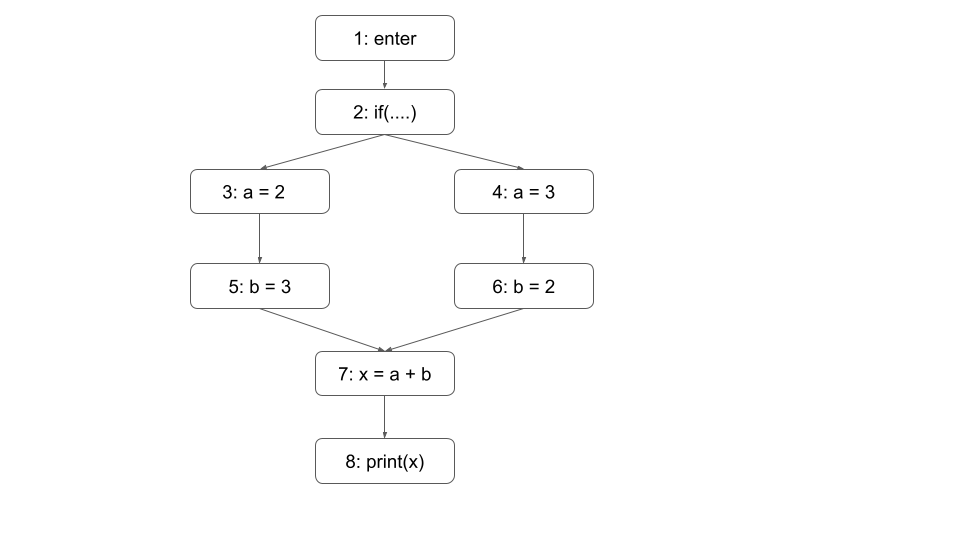
\includegraphics[width=0.8\textwidth]{p216.png}
	\caption{An example to illustrate that the
		solution computed by the iterative algorithm for constant propagation not equal to MOP.}
	\label{fig:p216}
\end{figure}


The MOP solution for the final \texttt{print} statement includes the pair $(x,5)$,
since $x$ is assigned the value $5$ on both paths to that statement. However,
the greatest solution to the set of equations for this program (the result
computed using the iterative algorithm) finds that $x$ is not constant at the
print statement. This is because the equations require that \texttt{\textit{n.before}} be the
meet of \texttt{m.after} for all predecessors \texttt{m}; in particular, they require that
the {\color{red} before} set for  \texttt{node 7 (x = a + b)}
has empty, since the {\color{red} after} sets
of the two predecessors have $(a,2), (b,3)$, and $(a,3), (b,2)$, respectively,
and the intersection of those two sets is empty. Given that value for
\texttt{7.before}, the equations require that \texttt{7.after} (and \texttt{8.before}) say that
$x$ is not constant. We can only discover that $x$ is constant after \texttt{node 7}
if both $a$ and $b$ are constant before \texttt{node 7}.




In 1977, a paper by Kam and Ullman\cite{kam1977monotone}
extended Kildall's results to show that, given monotonic dataflow functions:

\begin{itemize}
	\item The solutions to the set of equations form a lattice.
	\item The solution computed by the iterative algorithm is the greatest solution (using the lattice ordering).
	\item If the functions are monotonic but not distributive, then the solution computed by the iterative algorithm may be less than the MOP solution (using the lattice ordering).
\end{itemize}



\subsection{Speed of convergence}

Preorder means visit parents before children, it isalso called \textbf{reverse postorder(RPO)} . Postorder means visit children before parent.
RPO visits as many predecessors possible before visiting a node so in case of forward data flow problems (like Dominator computation) this would help to converge faster (as shown in Algorithm \ref{alg:Reverse Postorder}).




\begin{algorithm}[H]
	\caption{Depth-First Iterative Algorithm}\label{alg:Reverse Postorder}
	\begin{algorithmic}
		\State{{\color{blue}Step 1: depth-first post order}}
		\Function{main()}{}
		\State{{\color{blue}count} = 1;}
		\State{Visit({\color{blue}root});}
		\EndFunction

		\Function{Visit(n)}{}
		\For{{\color{blue}each successor s} that has {\color{blue}not been visited}}
		\State{{\color{green}PostOrder}(n) = {\color{blue}count};}
		\State{{\color{blue}count = count+1;}}
		\EndFor
		\EndFunction
		\State{{\color{blue}Step 2: reverse order}}
		\For{each node i}
		\State{{\color{red}rPostOrder}(i)= {\color{blue}NumNodes} - {\color{green}PostOrder(i)}}
		\EndFor
		\State{\color{blue}Step 3: Depth-First Iterate}
		\State{out[entry] = init\_value}
		\For{all nodes i}
		\State{out[i] = T}
		\EndFor
		\State{Change = True}
		\While{Change}
		\State{Change = False}
		\For{each node i {\color{red}in rPostOrder}}
		\State{in[i] = $\wedge$(out[p])}, for all predecessors p of i
		\State{oldout = out[i]}
		\State{out[i] = $f_i$ (in[i])}
		\If {oldout $\neq$ out[i]}
		\State{Change = True}
		\EndIf
		\EndFor
		\EndWhile
	\end{algorithmic}
\end{algorithm}


The number of passes are determined by number of back edges in the path essentially the nesting depth of the graph
\[
	\text{Number of iterations} = \text{number of back edges in any acyclic
		path} + 2
\]
in	real	programs,	average	of	2.75	


\subsection{Summary}
Let's answer the questions we asked before.
\begin{itemize}
	\item If D is a semi-lattice L which has finite descending chain, transfer function is monotone,
	      then the iterative algorithm will converge.
	\item  If dataflow framework is monotone,  then if the algorithm converges,
	      $IN[B] \preceq  MOP[B] $
	\item If dataflow framework is distributive, then if the algorithm converges,
	      $IN[B] = MOP[B]$
\end{itemize}


